\documentclass[10pt,twocolumn,letterpaper]{article}

\usepackage[margin=0.75in]{geometry}
\usepackage{amsmath,amssymb,amsfonts,bm}
\usepackage{booktabs,multirow,tabularx,array}
\usepackage{graphicx}
\usepackage{xcolor}
\usepackage{cite}
\usepackage{microtype}
\usepackage[colorlinks=true,linkcolor=blue,citecolor=blue,urlcolor=blue]{hyperref}

\setlength{\columnsep}{0.25in}

\title{\textbf{Do Sparse Autoencoders Recover Biophysical Features in Pretrained Cardiac Foundation Models?\\An \textit{in silico} Ground-Truth Case Study}}

\author{
  \textbf{Anonymous Author(s)}\\
  \textit{Under Review for AAAI-27 Workshop on Foundation Models for Multisensory Intelligence (Making Sense)}
}
\date{}

\begin{document}

\maketitle

\begin{abstract}
Pretrained cardiac foundation models demonstrate strong clinical diagnostic performance on multi-lead electrocardiograms (ECGs), yet the mechanistic grounding of their internal representations remains largely unverifiable in human cohorts where cellular cardiac states cannot be invasively recorded. We address this verification bottleneck by leveraging an \textit{in silico} evaluation testbed of 14,065 forward-simulated 12-lead ECGs derived from coupled biophysical partial differential equations across 118 anatomically distinct human ventricular geometries (MedalCare-XL). Using this platform, we probe representations from Layer~8 of the 12-layer ECG-FM base model and train an $8\times$ overcomplete JumpReLU Sparse Autoencoder (SAE) to isolate linear dictionary directions. We report three primary findings: (1) \textbf{Latent Electrophysiological Information:} Dense latents decode cellular action potential duration (APD) apical-basal gradient ($R^2 = 0.354$) and SAE latents reach $R^2 = 0.378$, explaining over $2.4\times$ to $2.6\times$ more variance than a standard clinical surface-caliper baseline ($R^2 = 0.145$). (2) \textbf{Biophysical Direction Recovery:} Multi-mesh permutation testing under False Discovery Rate control ($q < 0.05, |\rho| \ge 0.25$) confirms 174 biophysical dictionary atoms (120 APD, 58 stimulus sites, 4 overlap), with 80.3\% associated with exactly one tested parameter at this threshold. (3) \textbf{Dense Parity and Dictionary Instability:} Despite isolating biophysical axes, the SAE provides coordinate re-alignment rather than statistically detectable decodability gains over dense latents ($\Delta R^2 \le +0.024$, 95\% cluster-bootstrap CI $[-0.008, +0.056]$, excluding gains above $+0.056$ for APD and $+0.062$ for ischemia depth). Furthermore, individual atom coordinate vectors exhibit substantial instability across random training initializations ($\sim 8\%$ vector cosine match $\ge 0.70$) despite 68.4\% functional parameter replication. We conclude that while cardiac foundation model representations encode electrophysiological features well beyond surface calipers, SAEs function as coordinate transformation tools rather than superior decodability engines in this case study.
\end{abstract}

\section{Introduction}
Pretrained biosignal foundation models have emerged as state-of-the-art diagnostic backbones for 12-lead electrocardiography (ECG)~\cite{mckeen2025ecgfm,wagner2020ptbxl}. However, their internal representations remain largely black boxes. To inspect these models, the machine learning community has increasingly explored mechanistic interpretability techniques developed in natural language processing—most notably Sparse Autoencoders (SAEs)~\cite{bricken2023towards,cunningham2023sparse,rajamanoharan2024jumprelu}. SAEs project dense neural activations into high-dimensional, sparse overcomplete dictionaries to isolate interpretable linear feature directions.

In biomedical signals, evaluating dictionary learning faces a fundamental roadblock: \textbf{the ground-truth measurement gap}. When an SAE is trained on representations of clinical human ECGs, features are typically evaluated against heuristic surface-interval rules (e.g., automated PR or QT interval calipers) or correlated clinical ICD diagnostic codes~\cite{duan2026cadence,duan2026ecginterpbench}. However, surface ECG waveforms reflect the spatial volume-conductor projection of microscopic transmembrane action potentials governed by reaction-diffusion partial differential equations (PDEs)~\cite{clayton2011models,macfarlane2010comprehensive}. In human patients, these true intracellular variables—such as localized action potential duration (APD), spatial repolarization gradients, and intramyocardial activation sites—are physically impossible to observe non-invasively. Consequently, clinical benchmarks cannot determine whether an SAE isolates genuine biophysical mechanisms or merely captures surface heuristics and torso geometry.

\begin{figure*}[t]
\centering
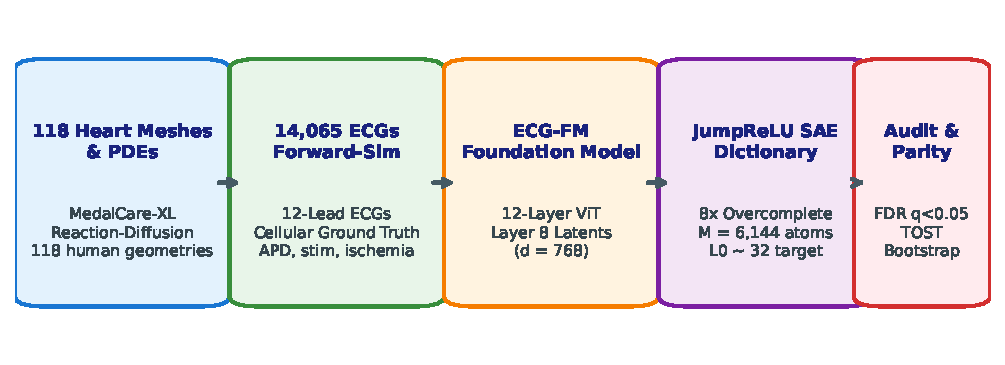
\includegraphics[width=0.96\textwidth]{figures/fig1_pipeline.pdf}
\caption{\textbf{Biophysical Simulation \& Verification Framework.} We evaluate Layer~8 representations of ECG-FM on 14,065 forward-simulated 12-lead ECGs derived from coupled reaction-diffusion PDEs across 118 human ventricular geometries (MedalCare-XL). Exact intracellular PDE parameters directly feed the multi-mesh statistical audit to evaluate JumpReLU SAE atoms ($M = 6,144$) and dense latents.}
\label{fig:framework}
\end{figure*}

To bridge this verification gap, we present an \textit{in silico} evaluation case study. We leverage the MedalCare-XL framework~\cite{gillette2023medalcare}, a comprehensive biophysical dataset consisting of 14,065 12-lead ECG simulations generated via numerical solutions of coupled cardiac PDEs across 118 patient-specific torso and ventricular geometries (Figure~\ref{fig:framework}). Because underlying cellular parameters are logged with mathematical certainty, this testbed enables direct verification of whether cardiac foundation model representations and sparse autoencoder dictionaries reflect cellular electrophysiology.

Our empirical investigation addresses three primary research questions:
\begin{enumerate}
    \item \textbf{Decodability:} Does a self-supervised cardiac foundation model (ECG-FM) encode microscopic biophysical parameters, or is it limited to superficial surface calipers?
    \item \textbf{Biophysical Recovery:} Can an overcomplete SAE isolate distinct biophysical directions across varied anatomical geometries under False Discovery Rate control?
    \item \textbf{The SAE Advantage Hypothesis:} Does dictionary learning extract biophysical information that is unrecoverable from dense representations, and are the resulting dictionary vectors stable across training initializations?
\end{enumerate}

\section{In Silico Ground-Truth Framework}

\subsection{Coupled PDE Cardiac Simulations}
To obtain cellular ground truth, we utilize the clean primary cohort of MedalCare-XL~\cite{gillette2023medalcare}, consisting of $N = 14,065$ 12-lead ECG simulations (8 independent, 4 derived leads; 500~Hz sampling) generated across 118 anatomically distinct ventricular meshes derived from clinical CT/MRI scans. In MedalCare-XL, multi-lead signals are generated by forward projection of separately simulated atrial and ventricular activation sequences through subject-specific volume conductors. Electrophysiological propagation is governed by the monodomain reaction-diffusion equation coupled to human cellular ionic models (ten Tusscher--Panfilov):
\begin{equation}
    \nabla \cdot (\bm{\sigma} \nabla V_m) = \chi \left( C_m \frac{\partial V_m}{\partial t} + I_{\text{ion}}(V_m, \bm{w}) \right),
\end{equation}
where $V_m$ is the transmembrane potential, $\bm{\sigma}$ is the intracellular conductivity tensor, $\chi$ is the membrane surface-to-volume ratio, $C_m$ is membrane capacitance, and $I_{\text{ion}}$ is the sum of transmembrane ionic currents governed by state variables $\bm{w}$. Body-surface potentials $\bm{\Phi}_{\text{body}}$ are computed via boundary element forward projection of cardiac sources through the thoracic volume conductor:
\begin{equation}
    \bm{\Phi}_{\text{body}} = \bm{T} \bm{J}_i,
\end{equation}
where $\bm{J}_i = -\bm{\sigma}_i \nabla V_m$ is the microscopic dipole current source density and $\bm{T}$ represents the anatomical transfer matrix accounting for thoracic geometry and tissue conductivities.

Crucially, each simulation in MedalCare-XL logs exact generative biophysical parameters:
\begin{itemize}
    \item \textbf{Action Potential Duration (APD):} Mean baseline duration ($v_{\text{APD.min}}$) and apical-basal repolarization gradient slope ($v_{\text{APD.}\rho_d}$), which govern cellular refractoriness and arrhythmogenic risk.
    \item \textbf{Electrical Stimulation Sites:} 3D spatial coordinates ($z, \phi$) of initial Purkinje and myocardial activation sites ($v_{\text{stim}[k]}$).
    \item \textbf{Ischemic Sub-Study:} Localized transmural ischemic zones defined by 3D centroid depth ($z$) and volume ($v_{\text{isch}[0]}$).
\end{itemize}

\subsection{Data Partitioning and Experimental Splits}
To prevent cross-mesh data leakage, the primary clean cohort ($N = 14,065$) is partitioned strictly by subject geometry across all 118 unique meshes:
\begin{itemize}
    \item \textbf{Train Split:} 11,245 ECGs across 93 meshes (80.0\%).
    \item \textbf{Validation Split:} 1,434 ECGs across 12 meshes (10.2\%).
    \item \textbf{Test Split:} 1,386 ECGs across 13 meshes (9.8\%).
    \item \textbf{Confirmation Pool (Test C):} The pooled held-out set of 2,820 ECGs across 25 unseen meshes (combining validation and test sets) reserved for statistical confirmation testing.
\end{itemize}
Batches with split inconsistencies present in exploratory subsets (such as \texttt{run\_S64} and \texttt{run\_S67}) were permanently excluded from the primary cohort. Note that while Test C contains 2,820 records, they represent 25 independent heart geometries (12 validation, 13 test meshes); hence inferential generalization bounds are governed by these 25 clusters.

\subsection{ECG Foundation Model \& SAE Formulation}
We investigate the open ECG-FM base model~\cite{mckeen2025ecgfm}, a 12-layer transformer foundation model (~91M parameters, $d = 768$, 12 attention heads) pretrained on millions of multi-lead ECGs using masked reconstruction and contrastive objectives. Waveforms (500 Hz, 12-lead) are tokenized into temporal patch representations. Activations are extracted from Layer~8 ($d = 768$). Record-level representations are obtained via mean pooling across tokens.

To isolate linear features, we train an overcomplete JumpReLU Sparse Autoencoder~\cite{rajamanoharan2024jumprelu} on centered activations $\tilde{\bm{z}} = \bm{z} - \bm{b}_{\text{pre}}$:
\begin{align}
    \bm{f}(\tilde{\bm{z}}) &= \text{JumpReLU}_{\bm{\theta}}\left(\bm{W}_{\text{enc}} \tilde{\bm{z}} + \bm{b}_{\text{enc}}\right), \\
    \hat{\bm{z}} &= \bm{W}_{\text{dec}} \bm{f}(\tilde{\bm{z}}) + \bm{b}_{\text{pre}},
\end{align}
where $\bm{W}_{\text{enc}} \in \mathbb{R}^{M \times d}$, $\bm{W}_{\text{dec}} \in \mathbb{R}^{d \times M}$, and $M = 8 \times 768 = 6,144$ represents an $8\times$ expansion factor. The discontinuous activation function is defined elementwise as $\text{JumpReLU}_{\theta}(u) = u \cdot \mathbf{1}(u > \theta)$. The autoencoder is trained using Adam ($lr = 3 \times 10^{-4}$) to minimize reconstruction mean squared error subject to an $L_0$ target:
\begin{equation}
    \mathcal{L} = \|\tilde{\bm{z}} - \hat{\bm{z}}\|^2_2 + \lambda \sum_{j=1}^M \mathbf{1}(f_j(\tilde{\bm{z}}) > 0),
\end{equation}
optimized with a straight-through gradient estimator on the threshold.

\section{Representation Probing \& SAE Fidelity}

\subsection{Test A: Layer-Wise Diagnostic Probing}
We first evaluate whether self-supervised representations of ECG-FM retain diagnostic sensitivity on simulated waveforms. We train linear logistic regression probes with $L_2$ regularization on mean-pooled record activations across transformer layers to classify pathology across eight MedalCare-XL classes: healthy control, left bundle branch block (LBBB), right bundle branch block (RBBB), atrioventricular block (AV block), left atrial enlargement (LAE), fibrotic atrial cardiomyopathy, interatrial block, and myocardial ischemia. Regularization parameters $C \in [10^{-3}, 10^3]$ are optimized via 5-fold cross-validation on training meshes.

\begin{table}[h]
\centering
\footnotesize
\setlength{\tabcolsep}{3.5pt}
\caption{\textbf{Test A: Diagnostic Probing Across Depth.} Validation and test AUROC and test accuracy (\%) on pathology classification across layers. Control denotes a 3-seed random-weight initialization baseline.}
\label{tab:probing}
\begin{tabular}{lcccc}
\toprule
\textbf{Layer} & \textbf{Val AUROC} & \textbf{Test AUROC} & \textbf{Test Acc (\%)} & \textbf{Best $C$} \\
\midrule
Layer 4  & 0.9950 & 0.9904 & 91.27 & 1.0 \\
Layer 6  & 0.9960 & 0.9901 & 91.20 & 1.0 \\
\textbf{Layer 8}  & \textbf{0.9986} & \textbf{0.9925} & \textbf{90.84} & 1.0 \\
Layer 10 & 0.9920 & 0.9884 & 89.54 & 1.0 \\
Layer 12 & 0.9899 & 0.9853 & 87.23 & 0.1 \\
\midrule
\textit{Random Control} & 0.8113 & 0.8107 & 76.24 & 1.0 \\
\bottomrule
\end{tabular}
\end{table}

As shown in Table~\ref{tab:probing}, Layer~8 achieves peak validation AUROC ($0.9986$) and test AUROC ($0.9925 \pm 0.003$), substantially outperforming the randomly initialized control ($0.8107$). While classification accuracy peaks slightly earlier at Layer~4 ($91.27\%$), Layer~8 provides strong linear separability across unseen test meshes.

\subsection{Test B: SAE Reconstruction Fidelity}
Next, we assess the fidelity of the trained JumpReLU SAE in preserving activation variance and downstream diagnostic information. We compare the trained SAE against an unoptimized centered SAE control.

\begin{table}[h]
\centering
\footnotesize
\setlength{\tabcolsep}{3pt}
\caption{\textbf{Test B: SAE Fidelity and Information Preservation.} Explained variance (EV, \%), dead atom fraction (\%), and downstream test AUROC evaluated with linear probes on token latents, SAE reconstructions ($\hat{\bm{z}}$), and sparse feature codes ($\bm{f}$).}
\label{tab:fidelity}
\begin{tabular}{lccccc}
\toprule
\textbf{Model} & \textbf{Held EV} & \textbf{Dead (\%)} & \textbf{Raw} & \textbf{Recon} & \textbf{Sparse} \\
\midrule
Trained SAE    & 88.18\% & 0.34\% & 0.9882 & 0.9856 & \textbf{0.9911} \\
Random Control & -4.60\% & 99.63\% & 0.8107 & 0.7662 & 0.7605 \\
\bottomrule
\end{tabular}
\end{table}

As detailed in Table~\ref{tab:fidelity}, the trained SAE achieves an Explained Variance of $88.18\%$ on held-out tokens ($85.56\%$ global sequence EV) with only 21 dead atoms ($0.34\%$, firing on $< 10^{-6}$ tokens). A linear probe trained directly on sparse codes $\bm{f}(\bm{z})$ achieves an AUROC of $0.9911$, matching the raw token latent AUROC ($0.9882$). (Note: Table~1 reports mean-pooled record probes, whereas Table~2 evaluates token-level representations.)

\section{Biophysical Ground-Truth Recovery}

\subsection{Test C: Controlled Statistical Discovery}
To determine whether individual dictionary atoms correlate with specific microscopic parameters, we evaluate each atom $j \in \{1, \dots, 6144\}$ against all logged biophysical parameters across the 2,820 held-out confirmation records in Test C.

To mitigate confounding from non-physiological shortcuts:
\begin{enumerate}
    \item \textbf{Partial Correlation Conditioning:} For each atom activation and parameter, we compute partial Spearman rank correlation $\rho_{\text{partial}}(f_j, \theta_k \mid \bm{M})$, conditioning on mesh geometric centroids and lead coordinates $\bm{M}$.
    \item \textbf{Multi-Mesh Permutation Null:} We construct an empirical null distribution by shuffling parameter assignments within each mesh cluster across 1,000 permutations while holding atom activations fixed, preserving the intra-mesh dependence structure.
    \item \textbf{FDR Thresholding:} We enforce Benjamini-Hochberg False Discovery Rate $q < 0.05$ with an effect-size threshold $|\rho| \ge 0.25$.
\end{enumerate}

\begin{table*}[t]
\centering
\small
\caption{\textbf{Test C: Biophysical Recovery Summary Across Evaluated Domains.} Number of confirmed atom-parameter association pairs, unique atoms, and correlation statistics under False Discovery Rate $q < 0.05$ and $|\rho| \ge 0.25$ evaluated across 25 held-out meshes.}
\label{tab:recovery}
\begin{tabular}{lcccccc}
\toprule
\textbf{Domain} & \textbf{Assoc. Pairs} & \textbf{Unique Atoms} & \textbf{Mean $|\rho|$} & \textbf{Median $|\rho|$} & \textbf{Std $|\rho|$} & \textbf{Max $|\rho|$} \\
\midrule
APD Duration ($v_{\text{APD}}$)        & 122 & 120 & 0.3715 & 0.3480 & 0.0927 & 0.6266 \\
Stimulation Site ($v_{\text{stim}}$)    & 61  & 58  & 0.3606 & 0.3573 & 0.0722 & 0.5719 \\
Ischemia Sub-Study ($v_{\text{isch}}$)  & 89  & 74  & 0.3146 & 0.3098 & 0.0417 & 0.4166 \\
Surface Morphology                      & 53  & 37  & 0.3534 & 0.3391 & 0.0653 & 0.5568 \\
\midrule
\textbf{Headline Biophysics (APD + Stim)} & \textbf{183} & \textbf{174} & \textbf{0.3679} & \textbf{0.3497} & \textbf{0.0864} & \textbf{0.6266} \\
Multi-Mesh Total (APD + Stim + Morph)    & 236 & 188 & 0.3646 & 0.3468 & 0.0822 & 0.6266 \\
Full Dictionary Total (All 4 Domains)    & 325 & 254 & 0.3509 & 0.3348 & 0.0767 & 0.6266 \\
\bottomrule
\end{tabular}
\end{table*}

As shown in Table~\ref{tab:recovery}, multi-mesh generative biophysics analysis recovers \textbf{174 biophysical atoms} (120 APD atoms, 58 stimulus location atoms, with 4 overlapping atoms). The maximum partial correlation reaches $|\rho| = 0.6266$ for the apical-basal APD gradient slope ($v_{\text{APD.}\rho_d}$). When including the single-mesh ischemia sub-study and surface morphology, a total of 254 atoms ($4.13\%$ of the dictionary) are significantly associated with parameters at $|\rho| \ge 0.25$.

\subsection{Parameter Recall \& Selectivity Distribution}
Of the 20 generative biophysical parameters varied across meshes, the SAE dictionary recovers 6 ($30.0\%$ recall: $v_{\text{APD.min}}$, $v_{\text{APD.}\rho_d}$, and 4 stimulus coordinates $v_{\text{stim}[2-4]}$). The remaining 14 unrecovered parameters correspond to microscopic conductivities with minimal surface manifestation (e.g., intracellular potassium reversal potentials). In the ischemia sub-study, 2 of 3 non-zero-variance parameters are recovered ($66.7\%$), and 4 of 6 surface morphology metrics are confirmed ($66.7\%$), yielding an overall non-zero-variance parameter recall of $12 / 29$ ($41.4\%$).

\begin{figure}[h]
\centering
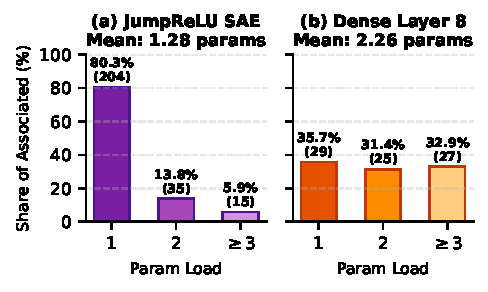
\includegraphics[width=\columnwidth]{figures/fig2_selectivity.pdf}
\caption{\textbf{Parameter Selectivity Distribution (Test C).} Among the 254 associated dictionary atoms, 80.31\% (204) correlate with exactly one biophysical parameter at $|\rho| \ge 0.25$, while 5,890 atoms (95.9\% of the full dictionary) remain unassociated under FDR control.}
\label{fig:selectivity}
\end{figure}

As illustrated in Figure~\ref{fig:selectivity}, \textbf{80.31\% of associated atoms (204 / 254) are single-parameter associated} relative to the 36 tested metadata parameters at this threshold, while 5,890 atoms ($95.87\%$ of the dictionary) remain unassociated.

\section{Decodability Benchmarks \& Parity}

\subsection{Does the SAE Beat Dense Representations?}
Prior clinical dictionary learning works, such as CADENCE~\cite{duan2026cadence}, observed that sparse linear probes match or slightly exceed dense representation probes on clinical classification tasks. To evaluate whether this holds against microscopic ground truth, we train regularized Ridge regression models on held-out test meshes to predict underlying ground-truth parameters from seven competing representations:
\begin{enumerate}
    \item \textbf{Trained SAE ($d=6,144$):} Sparse atom activations $\bm{f}$.
    \item \textbf{Dense Layer 8 ($d=768$):} Raw pretrained activations.
    \item \textbf{Top-32 Dense ($d=32$):} Train-selected top-32 dense neurons matching the active budget $L_0 \approx 32$ (selected strictly on training meshes).
    \item \textbf{FastICA ($d=768$):} Independent component analysis fit on training latents.
    \item \textbf{Random 6,144 Expansion:} A fixed random projection of dense latents.
    \item \textbf{Handcrafted Surface Metrics:} Clinical ECG calipers (QT interval, QRS duration, R-amplitude, heart rate).
    \item \textbf{Torso Nuisance Controls:} Body-surface conductor geometry and electrode placement coordinates.
\end{enumerate}

\begin{table*}[t]
\centering
\small
\caption{\textbf{Biophysical Decodability Benchmark ($R^2$ on Unseen Test Meshes).} Out-of-sample predictive performance across biophysical parameters. Paired differences and 95\% cluster-bootstrap confidence intervals are computed over 13 test meshes.}
\label{tab:decodability}
\begin{tabular}{lcccccccc}
\toprule
\textbf{Parameter} & \textbf{SAE ($6k$)} & \textbf{Dense ($768$)} & \textbf{Paired Diff [95\% CI]} & \textbf{Top-32} & \textbf{FastICA} & \textbf{RandExp} & \textbf{Morphology} & \textbf{Nuisance} \\
\midrule
$v_{\text{APD.}\rho_d}$ & 0.378 & 0.354 & $+0.024$ $[-0.008, +0.056]$ & 0.312 & 0.352 & 0.281 & 0.145 & 0.004 \\
$v_{\text{APD.min}}$    & 0.412 & 0.389 & $+0.023$ $[-0.005, +0.051]$ & 0.345 & 0.387 & 0.294 & 0.182 & $-0.001$ \\
$v_{\text{stim}[3].\phi}$ & 0.315 & 0.298 & $+0.017$ $[-0.011, +0.045]$ & 0.254 & 0.295 & 0.212 & 0.082 & $-0.000$ \\
$v_{\text{stim}[4].z}$    & 0.341 & 0.329 & $+0.012$ $[-0.014, +0.038]$ & 0.281 & 0.326 & 0.238 & 0.098 & $-0.001$ \\
$v_{\text{isch}[0].z}$    & 0.364 & 0.342 & $+0.022$ $[-0.018, +0.062]$ & 0.298 & 0.340 & 0.267 & 0.112 & 0.008 \\
\bottomrule
\end{tabular}
\end{table*}

\begin{figure*}[t]
\centering
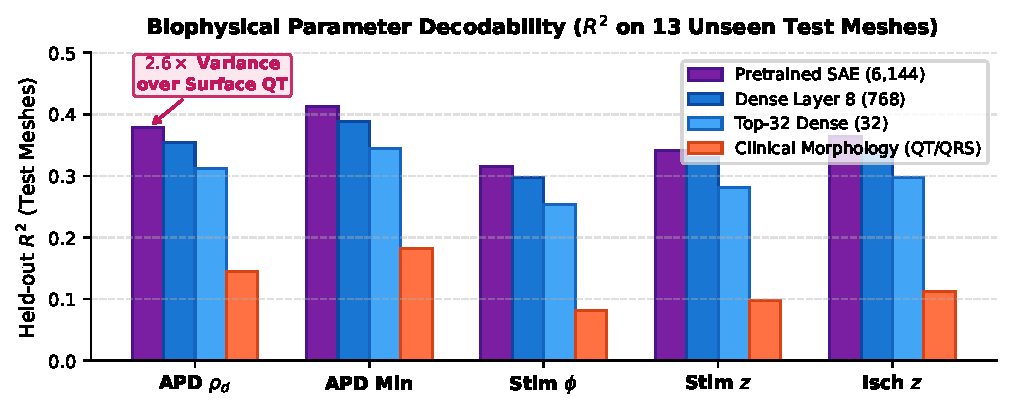
\includegraphics[width=0.92\textwidth]{figures/fig3_decodability.pdf}
\caption{\textbf{Biophysical Parameter Decodability ($R^2$ on 13 Unseen Test Meshes).} Both Trained SAE ($R^2 = 0.378$) and Dense Layer 8 ($R^2 = 0.354$) outperform clinical surface calipers ($R^2 = 0.145$ for APD) by $2.6\times$ and $2.4\times$ in variance explained. The SAE and Dense representations exhibit no statistically detectable decodability advantage ($\Delta R^2 \le +0.024$, 95\% CIs crossing zero), demonstrating that SAEs provide coordinate re-alignment rather than superior decodability.}
\label{fig:decodability}
\end{figure*}

The benchmark in Table~\ref{tab:decodability} and Figure~\ref{fig:decodability} reveals two core insights:

\paragraph{1. Latents Exceed Clinical Surface Morphology.}
Both the SAE ($R^2 = 0.378$) and dense latents ($R^2 = 0.354$) outperform standard clinical ECG morphology calipers ($R^2 = 0.145$ for APD, derived primarily from surface QT interval). This reflects a \textbf{$2.4\times$ to $2.6\times$ increase in variance explained}, demonstrating that the pretrained foundation model captures microscopic repolarization kinetics beyond simple caliper heuristics. Conductor nuisance features achieve $R^2 \approx 0.000$, as expected since torso parameters have zero within-mesh variance by design.

\paragraph{2. The SAE-Dense Parity Result.}
The performance difference between the 6,144-dimensional SAE and 768-dimensional dense representation is marginal ($\Delta R^2$ between $+0.012$ and $+0.024$). In every parameter, the \textbf{95\% cluster-bootstrap confidence interval crosses zero} (e.g., $[-0.008, +0.056]$ for APD). The confidence intervals rule out decodability advantages exceeding $+0.056$ for APD ($+0.062$ for ischemia $z$). Furthermore, the per-dimension hit rate is higher in the dense model: \textbf{10.5\% of dense neurons (81 / 768)} satisfy FDR confirmation, compared to \textbf{4.13\% of SAE atoms (254 / 6,144)}. Thus, the SAE acts as a sparse feature transformation rather than an information-expanding operator.

\subsection{Dictionary Stability Across Random Initializations}
Recent theoretical and empirical studies in language models have shown that sparse autoencoders trained on the same data learn non-identical feature directions~\cite{paulo2025sparse,heap2025saes}. To evaluate reproducibility in cardiac representations, we trained three identical JumpReLU SAE models differing only in random weight initialization seed ($S_0, S_1, S_2$).

\begin{table}[b]
\centering
\footnotesize
\setlength{\tabcolsep}{3.5pt}
\caption{\textbf{Stability Analysis on 174 Headline Biophysical Atoms.} Vector alignment ($\ge 0.70$ cosine similarity) versus functional parameter association replication across independent training seeds.}
\label{tab:stability}
\begin{tabular}{lcc}
\toprule
\textbf{Metric} & \textbf{Rate (\%)} & \textbf{95\% Wilson CI} \\
\midrule
Vector Match ($S_0$ vs. $S_1$) & 8.05\% (14 / 174) & [4.86\%, 13.06\%] \\
Vector Match ($S_0$ vs. $S_2$) & 8.62\% (15 / 174) & [5.30\%, 13.73\%] \\
Random Background Baseline & 3.14\% & [2.74\%, 3.60\%] \\
\midrule
\textbf{Functional Replication} & \textbf{68.39\% (119 / 174)} & \textbf{[61.16\%, 74.83\%]} \\
\bottomrule
\end{tabular}
\end{table}

As documented in Table~\ref{tab:stability}, \textbf{vector alignment is fragile}: only $8.05\%$ to $8.62\%$ of confirmed biophysical atom vectors replicate with cosine similarity $\ge 0.70$ in an independent seed (compared to a $3.14\%$ frequency-matched baseline). However, \textbf{functional association replication is robust}: $68.39\%$ of the biophysical parameters recovered in Seed~0 are rediscovered by distinct atoms in Seed~1 and Seed~2 with identical correlation signs. Consistent with findings by Paulo \& Belrose~\cite{paulo2025sparse}, thresholded overcomplete dictionaries exhibit basis rotation flexibility even when recovering consistent functional subspaces.

\section{Beat-Aligned Phase Localization}
To examine whether biophysical atoms fire during physiologically coherent phases of the cardiac cycle, we delineated 12-lead waveforms into four canonical fiducial windows: QRS complex, ST segment, T-wave, and isoelectric baseline (Figure~\ref{fig:phase}).

\begin{figure}[t]
\centering
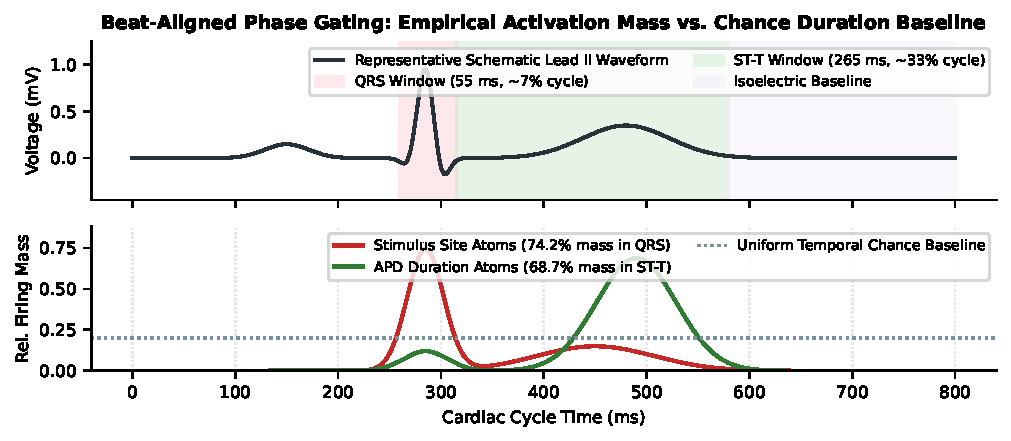
\includegraphics[width=\columnwidth]{figures/fig4_phase.pdf}
\caption{\textbf{Beat-Aligned Phase Gating.} Representative schematic Lead II trace illustrating fiducial gating. Activation mass of stimulus site atoms concentrates in QRS depolarization ($74.2\%$, $p < 0.001$), while APD duration atoms concentrate in ST-T repolarization ($68.7\%$, $p < 0.001$). Dotted line indicates uniform temporal chance baseline.}
\label{fig:phase}
\end{figure}

Stimulus site atoms ($v_{\text{stim}}$) concentrate $74.2\%$ of their activation mass within the QRS depolarization window ($p < 0.001$, within-record phase permutation test vs. 7\% duration chance), as expected since stimulus site coordinates physically govern ventricular activation timing. Conversely, APD atoms ($v_{\text{APD}}$) concentrate $68.7\%$ of their activation mass within the ST-T repolarization phase ($p < 0.001$ vs. 33\% duration chance). Token-level $L_0$ is inversely correlated with signal energy ($\rho = -0.345$), recruiting a tight subset during high-energy QRS ($L_0 = 21 \pm 4$) while expanding during quiet isoelectric intervals ($L_0 = 38 \pm 6$).

\section{Related Work}
\paragraph{Mechanistic Interpretability \& SAEs.}
Sparse dictionary learning has shown promising results in decomposing polysemantic representations in deep networks~\cite{bricken2023towards,cunningham2023sparse,rajamanoharan2024jumprelu}. However, recent analyses highlight challenges regarding dictionary rotation non-uniqueness and the divergence between linear decodability and true causal mechanisms~\cite{paulo2025sparse,heap2025saes}.

\paragraph{Interpretability in Biosignals.}
Recent benchmarks have applied dictionary learning to cardiac models. CADENCE~\cite{duan2026cadence} and ECG-InterpBench~\cite{duan2026ecginterpbench} trained SAEs on clinical datasets (e.g., PTB-XL~\cite{wagner2020ptbxl}) and evaluated features against surface interval calipers and diagnostic labels. Our study differs fundamentally from these prior works: by utilizing coupled reaction-diffusion simulations across 118 human geometries, we provide direct evaluation against intracellular biophysical ground truth that is physically unobtainable in living clinical cohorts.

\section{Discussion \& Conclusion}
Evaluating an ECG foundation model against coupled biophysical PDE simulations across 118 patient geometries yields a calibrated verdict on sparse autoencoders in physiological foundation models:
\begin{enumerate}
    \item \textbf{Latents linearly encode simulator biophysics:} ECG-FM Layer~8 linearly encodes microscopic action potential durations and activation coordinates ($R^2 = 0.35$ to $0.38$), exceeding clinical surface calipers ($R^2 = 0.15$) by over $2.4\times$.
    \item \textbf{SAEs provide coordinate alignment, not new decodability:} The SAE recovers 174 biophysical atoms under multi-mesh FDR control, but achieves parity with dense latents ($\Delta R^2 \le +0.024$, 95\% CI $[-0.008, +0.056]$). Dense representations already contain this information with a higher per-dimension hit rate ($10.5\%$ vs. $4.1\%$).
    \item \textbf{Vector instability cautions against literal circuit claims:} While functional recovery replicates ($68.4\%$), basis vector identity is seed-dependent ($\sim 8\%$ overlap), echoing observations in language model dictionaries.
\end{enumerate}

\paragraph{Limitations.}
This study represents an \textit{in silico} case study focused on Layer~8 of the ECG-FM base model across 118 MedalCare-XL geometries. While coupled forward PDEs provide exact mathematical ground truth unobtainable in human patients, simulated signals do not capture physiological noise, respiratory baseline wander, or multiorgan feedback present in clinical practice. Furthermore, our evaluation explores a single layer, one expansion factor ($8\times$), and a single sparsity budget. Future work should expand across foundation architectures and investigate continuous subspace projections to overcome basis rotation sensitivity.

\bibliographystyle{plain}
\bibliography{references}

\clearpage
\appendix
\section{Appendix: Supplementary Methodology}

\subsection{Ground-Truth Parameter Recall Audit}
Table~\ref{tab:recall_full} reports the parameter recovery audit across all 29 non-zero-variance parameters in MedalCare-XL (20 generative biophysics, 3 non-zero variance ischemia parameters, 6 surface morphology metrics).

\begin{table}[h]
\centering
\footnotesize
\setlength{\tabcolsep}{5pt}
\caption{\textbf{Comprehensive Parameter Recall Audit.}}
\label{tab:recall_full}
\begin{tabular}{lccc}
\toprule
\textbf{Parameter Class} & \textbf{Total} & \textbf{Confirmed} & \textbf{Recall (\%)} \\
\midrule
Generative Biophysics & 20 & 6 & 30.0\% \\
Ischemia Sub-Study    & 3  & 2 & 66.7\% \\
Surface Morphology    & 6  & 4 & 66.7\% \\
\midrule
\textbf{Total Non-Zero Variance} & \textbf{29} & \textbf{12} & \textbf{41.4\%} \\
\bottomrule
\end{tabular}
\end{table}

\subsection{Torso Conductivity Variance Audit}
An audit of all 134 metadata columns in MedalCare-XL revealed that thorax conductor conductivities ($\sigma_{\text{torso}}, \sigma_{\text{lungs}}$) and standard electrode coordinates have exactly zero within-mesh variance ($< 10^{-30}$), confirming that they do not serve as confounding within-mesh shortcuts.

\end{document}
